\section{Tracking}\label{sec:tracking}

To maintain continuous trajectories across frames, the tracking framework evolves from a purely spatial baseline to an architecture robust to appearance variation.
As a baseline, we employ Simple Online and Realtime Tracking (SORT) \cite{sort}, which propagates tracks using a Kalman filter and associates predicted boxes to incoming detections via the Hungarian algorithm using Intersection-over-Union (IoU) overlap.
SORT's reliance on spatial overlap, however, leads to frequent identity switches when players cross paths.

% This section progresses from the SORT baseline to a DeepSORT tracker with several
% robustness mechanisms, and finally to a label resolution step.

% \subsection{Simple Online and Realtime Tracking (SORT)}
% As a baseline tracker, we adopt Simple Online and Realtime Tracking (SORT) \cite{sort}.
% Each track is propagated forward by a Kalman filter under a constant-velocity motion model, and the predicted boxes are associated to the new detections via the Hungarian algorithm, using spatial overlap (IoU) as the matching cost.

% Its main limitation is that it relies on proximity alone, with no notion of appearance: when two players cross, their predicted boxes overlap and the tracker frequently swaps their identities.

\subsection{DeepSORT}
Our tracking framework adopts DeepSORT \cite{deepsort} to reduce identity swaps by augmenting the Kalman-filter motion model with appearance information.
For each detection, a lightweight \emph{OSNet} \cite{reid} produces an appearance embedding that is appended to a per-track rolling gallery.
Association is performed by a matching cascade that prioritizes appearance similarity before spatial overlap.

Building on this foundation, we introduce several improvements.
The \textbf{Confidence-Aware Kalman Update (NSA)} reduces state-correction jitter by scaling the measurement covariance according to detection confidence rather than treating all bounding-box updates equally.
\textbf{Low-Confidence Recovery (ByteTrack)} \cite{bytetrack} performs a second-pass association between unmatched tracks and low-confidence detections using spatial overlap, preserving continuity through partial occlusions.
\textbf{Track Resurrection} addresses prolonged occlusions by retaining the appearance galleries of recently terminated tracks for a brief temporal window; when a newly detected player closely matches a retained gallery, the original identity is restored rather than initializing a new track.
Finally, \textbf{Coasting} bridges short gaps by emitting a track's Kalman-predicted position while it remains unmatched, provided the prediction remains within frame bounds and does not overlap an already-assigned bounding box.

A final \textbf{Label Resolution} step unifies the detector's per-frame class predictions across each trajectory.
Each track is assigned its confidence-weighted majority label; identity conflicts between tracks are resolved in favor of the higher-confidence prediction.
The ball category is exempt from unique-identity arbitration.

% \subsubsection{Confidence-Aware Kalman Update (NSA)}
% Standard Kalman filtering weighs all bounding box updates uniformly during state correction.
% To minimize tracking jitter, we scale the measurement covariance by the detection confidence, ensuring high-confidence detections exhibit greater influence than uncertain ones.

% \subsubsection{Low-Confidence Recovery (ByteTrack)}
% Low-confidence detections often represent genuine players experiencing transient occlusion or motion blur.
% Adopting the ByteTrack \cite{bytetrack} paradigm, unmatched tracks are given a second-pass association against these low-confidence boxes based strictly on spatial overlap.
% This recovery mechanism maintains track continuity through partial occlusions; however, to prevent gallery corruption from noisy bounding boxes, these detections are excluded from appearance embedding updates.

% \subsubsection{Track Resurrection}
% When a trajectory is lost due to prolonged occlusion, standard trackers terminate the track, causing a re-emerging player to receive a new identity.
% We retain appearance galleries of recently terminated tracks for a short temporal window and restore an original identity when a new detection closely matches a retained gallery.

% \subsubsection{Coasting}
% When a track is momentarily left unmatched, it continues to report its Kalman-predicted box so that short gaps are bridged, provided this prediction remains within the frame and does not overlap a box already assigned to another track.

% \subsection{Label Resolution}
% Because the fine-tuned detector assigns unique class labels to individual player identities, a single trajectory may accumulate conflicting class predictions across frames.
% To resolve this, each track is assigned its confidence-weighted majority label, with any identity claimed by two tracks kept by the more confident one and the other taking its next-best label.
% The ball class is exempt from this arbitration procedure, as it represents a global category rather than a mutually exclusive unique identity.

\begin{figure}[h]
  \centering
  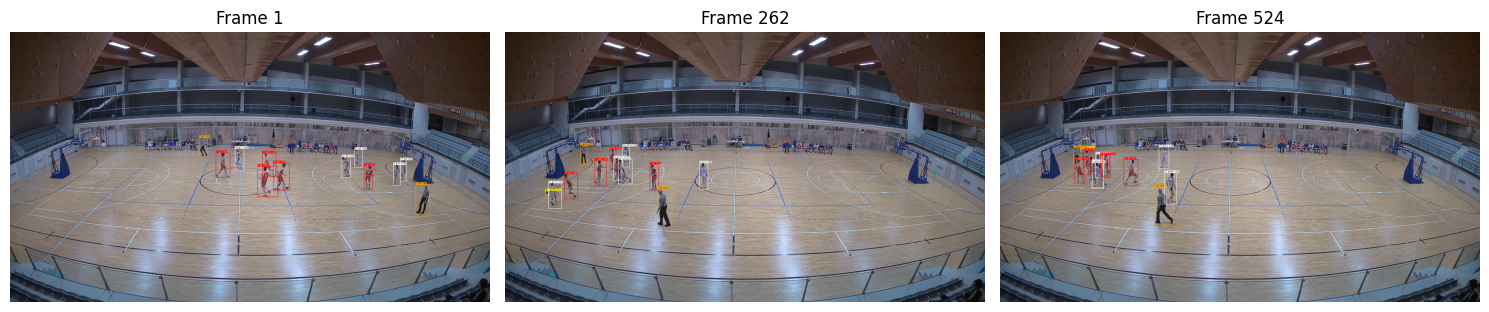
\includegraphics[width=\linewidth]{../assets/media/fig_tracking.png}
  \caption{Sample tracking output from DeepSORT on cam\_13.}
\end{figure}